\documentclass[letterpaper,12pt]{scrartcl}
\usepackage{epsfig,latexsym,amsmath,amssymb,epic,eepic,psfrag,subfigure,float,euscript,array}
\usepackage[latin1]{inputenc}
\usepackage[margin=24mm]{geometry}
\usepackage{tikz,pgf,pgfplots}
\usepgfplotslibrary{fillbetween}
\usepgfplotslibrary{groupplots}
\usetikzlibrary{decorations, arrows, fit, circuits.plc.ladder}

\usepackage[amssymb]{SIunits}

\newenvironment{exercise}[1][Exercise]{\begin{trivlist} \item[\hskip
    \labelsep {\stepcounter{exerctr}\bfseries #1
      \arabic{exerctr}}]}{\end{trivlist}\vspace{10mm}}

\newcounter{exerctr}
\newcounter{abcctr}[exerctr]

\newcommand{\abc}{\noindent\vspace{1mm}\\ \textbf{
    \stepcounter{abcctr}(\alph{abcctr})\ }}
\newcommand{\bbm}{\begin{bmatrix}}
\newcommand{\ebm}{\end{bmatrix}}
\newcommand{\point}[1]{\hfill \textbf{ (#1p)}\\ \vspace{-5mm}}
\newcommand{\ctrb}{\EuScript{S}}
\newcommand{\Lap}{\mathcal{L}}
\newcommand{\obsv}{\EuScript{O}}
\newcommand{\realdel}{\text{Re}}
\newcommand{\imagdel}{\text{Im}}
\newcommand{\bC}{\mathbb{C}}
\newcommand{\bR}{\mathbb{R}}
\newcommand{\bmpv}{\begin{minipage}[t]}
\newcommand{\bmps}{\begin{minipage}[t]{45mm}}
\newcommand{\bmpm}{\begin{minipage}[t]{90mm}}
\newcommand{\bmpl}{\begin{minipage}[t]{\textwidth}}
\newcommand{\emp}{\end{minipage}}
\newcommand{\mexp}[1]{\ensuremath{\mathrm{e}^{#1}}}

\newcommand{\AxisRotator}[1][rotate=0]{%
    \tikz [x=0.2cm,y=0.60cm,line width=.1ex,-stealth,#1] \draw (0,0) arc (-150:150:1 and 1);%
}

%\addtolength{\topmargin}{-1cm}
%\textheight 22.5cm
%\oddsidemargin 1.3cm
%\evensidemargin 1.3cm

\makeatletter
\newcommand*{\rom}[1]{\expandafter\@slowromancap\romannumeral #1@}
\makeatother

\newcommand*\circled[1]{\tikz[baseline=(char.base)]{
            \node[shape=circle,draw,inner sep=2pt] (char) {#1};}}


\title{Modeling and automation - Evidence 1}
\author{Kjartan Halvorsen}
\date{}

\begin{document}

\maketitle


\begin{description}
\item[Time] Thursday January 26 2023
\item[Place] 4102
\item[Permitted aids] The single page with your own notes.
\end{description}

All answers should be readable and well motivated (if nothing else is written). Solutions/motivations should be written on the provided spaces in this exam. Use the last page if more space is needed.

\begin{center}
{\Large Good luck!} \\
\end{center}

\noindent
\fbox{
\bmpl
\textbf{ Matricula and name:}\\
\vspace*{14mm}
\emp}


%\clearpage
\section*{Yaw control of a wind turbine}
Yaw is the horizontal angle between the direction the wind is blowing from and the direction the wind turbine is facing. Most wind turbines in commercial use have active control of the yaw angle in order to optimize energy production. \begin{center}
  \begin{tikzpicture}[node distance = 2cm]
    \node (image) {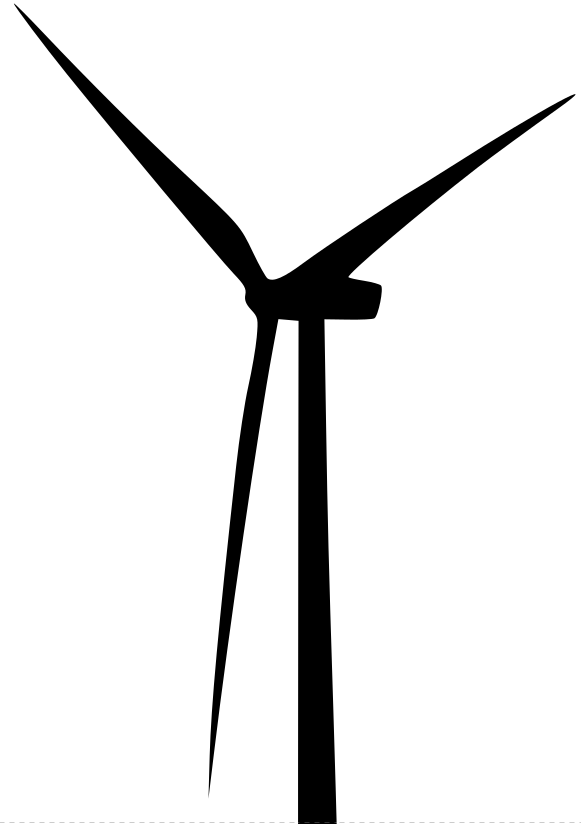
\includegraphics[width=0.2\linewidth]{../figures/wind-turbine-top.png}};
    \draw[->, thick, black!80!red!70] (1,0.65) -- node[coordinate, pos=0.8] (heading) {} (-3.4,0.65);
    \draw[->, thick, black!80!blue!70] (0.8,0.89) -- node[coordinate, pos=0.8] (winddir) {} (-2.7,-0.3);
    \draw[<-,] (heading) to[out=-135, in=150] node[left] {$y(t)$} (winddir);

    \node[coordinate, right of=image, node distance=5cm] (input) {};
    \node[circle, draw, inner sep=1pt, right of=input, ] (sum) {\small $\Sigma$};
    \node[draw, right of=sum, minimum height=12mm, minimum width=16mm] (block) {$G(s)$};
    \node[coordinate, right of=block] (output) {};
    \node[coordinate, above of=sum, node distance=14mm] (disturbance) {};
    
    \draw[->] (input) -- node[above, near start] {$u(t)$} (sum);
    \draw[->] (disturbance) -- node[left, near start] {$v(t)$} (sum);
    \draw[->] (sum) -- node[left, near start] {$$} (block);
    \draw[->] (block) -- node[above, near end] {$y(t)$} (output);
  \end{tikzpicture}
\end{center}
Assume that the friction force opposing the turning of the turbine is viscuous (proportional to the velocity), and that the wind force is causing a disturbance torque on the head. The dynamics of the system can then be described by the differential equation
\begin{equation}
 J\ddot{y}(t) + f\dot{y}(t) = u(t) + v(t),
\label{eq:odeyaw}
\end{equation}
where $y(t)$ is the yaw angle, $u(t)$ is the torque produced by the motor turning the head, $v(t)$ is the disturbance torque, $J$ is the moment of inertia and $f$ is the friction coefficient.

\subsection*{Problems}
\begin{exercise}

\abc
Show that the plant model \eqref{eq:odeyaw} can be expressed in the Laplace-domain as
\[ Y(s) = G(s)\big(U(s) + V(s)\big) = \frac{b}{s(s+a)} \big( U(s) + V(s)\big), \] 
with $b = \frac{1}{J}$ and $a = \frac{f}{J}$. 

\noindent
\fbox{
\bmpl
\textbf{Calculations:}\\
\vspace*{75mm}
\emp}

\abc Determine the poles of the system

\noindent
\fbox{
\bmpl
\textbf{Calculations:}\\
\vspace*{45mm}
\emp}

\abc
Choose a state vector $x$, and write the system \eqref{eq:odeyaw} on state-space form.
\begin{align*}
  \dot{x} &= Ax + B \bbm u\\v \ebm \\
  y &= Cx
\end{align*}
Note that $B$ is a matrix with two columns, \(B = \bbm B_1 & B_2\ebm,\) so an equivalent way of writing the state-space model is
\begin{align*}
  \dot{x} &= Ax + B_1 u + B_2v \\
  y &= Cx
\end{align*}


\noindent
\fbox{
\bmpl
\textbf{Calculations:}\\
\vspace*{82mm}
\emp}


\end{exercise}

\section*{A spring-mass system}


The figure below shows a system consisting of one  mass connected with two \textbf{identical} springs to two rigid walls. The mass can move without friction in the horizontal direction.
\begin{center}
  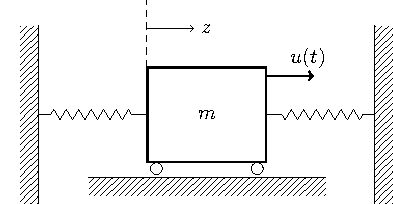
\includegraphics[width=0.45\linewidth]{../figures/one-mass-two-springs}
\end{center}
The displacement $z$ is a deviation from the equilibrium position when the mass is in the middle position between the two walls. There is an external force $u(t)$ acting on the mass. 

\begin{exercise}

\abc
Draw a free-body diagram.

\noindent
\fbox{
\bmpl
\textbf{ Drawing:}\\
\vspace*{50mm}
\emp}

\abc
The spring is nonlinear, and the magnitude of the force in the spring is given by
\[ F_s = a_1x + a_2 x^3,\] where $x$ is the deviation from its resting length. When the mass is in equilibrium, the two springs are stretched the same amount $x_0$ (since they are identical). The corresponding forces in the two springs is $F_0$ (the two forces are of the same magnitude but have opposite direction). \textbf{Determine the parameter $k$ in a linear model of the spring}
\[ F(t) = k\,z(t), \]
where $z(t)$ and $F(t)$ are deviation variables,  i.e. $x(t) = x_0 + z(t)$ and $F_s(t) = F_0 + F(t)$.


\noindent
\fbox{
\bmpl
\textbf{ Calculations:}\\
\vspace*{60mm}
\emp}

\abc
What are the dimensions in SI-units of the parameters $k$,  $a_1$ and $a_2$ respectively? 

\noindent
\fbox{
  \bmpl
  \vspace*{3mm}
\textbf{ $[k] = $}\\[1mm]
\textbf{ $[a_1] = $}\\[1mm]
\textbf{ $[a_2] = $}\\[1mm]
\emp}
'
\abc
Determine the differential equation that describes the system.

\noindent
\fbox{
\bmpl
\textbf{ Calculations:}\\
\vspace*{100mm}
\emp}

\end{exercise}

\cleardoublepage
\end{document}
\section*{Solutions}
\setcounter{exerctr}{0} 

\subsection*{Wind turbine}

\begin{exercise}
  \abc
  Since we are interested in the transfer function only, not the response to initial values, we set all initial values to zero when applying the Laplace transform to \eqref{eq:odeyaw}. This gives
  \[Js^2Y(s) + fsY(s) = U(s) + V(s)\]
  solving for Y(s) gives
  \[ Y(s) = \frac{\frac{1}{J}}{s(s+\frac{f}{J})} U(s) + \frac{\frac{1}{J}}{s(s+\frac{f}{J})}V(s) = \frac{\frac{1}{J}}{s(s+\frac{f}{J})}(U(s) + V(s)) \]

  \abc
  One suitable choice of state vector is
  \[ x = \bbm y\\\dot{y} \ebm, \]
  which gives the model
  \begin{align*}
    \dot{x}_1 &= \dot{y} = x_2\\
    \dot{x}_2 &= -\frac{f}{J}\dot{y} + \frac{1}{J} u + \frac{1}{J} v = -\frac{f}{J}x_2 + \frac{1}{J}u + \frac{1}{J} v
  \end{align*}
  which can be written
  \begin{align*}
    \dot{x} &= \bbm 0 & 1\\0 & -\frac{f}{J} \ebm x + \bbm 0 & 0 \\\frac{1}{J} & \frac{1}{J}  \ebm \bbm u\\v\ebm.\\
    y &= \bbm 1 & 0 \ebm x.
  \end{align*}

\end{exercise}

\subsection*{Spring-mass system}

\begin{exercise}
  \abc
  Free-body-diagrams of the two bodies gives
  \begin{center}
    \begin{tikzpicture}
      \node[draw, minimum height=14mm, minimum width=14mm] (m1) {M};
      \draw[->] (m1.west) -- ++(-14mm, 0) node[below] {$F_{s_1}$};
      \draw[<-] (m1.north west) -- ++(-14mm, 0) node[above] {$F$};
      \draw[<-] (m1.east) -- ++(14mm, 0) node[above] {$F_{s_2}$};

      \begin{scope}[xshift = 6cm]
      \node[draw, minimum height=14mm, minimum width=14mm] (m2) {M};
      \draw[<-] (m2.west) -- ++(-14mm, 0) node[above] {$F_{s_2}$};
      \draw[<-] (m2.east) -- ++(14mm, 0) node[above] {$F_{d}$};
      \end{scope}
    \end{tikzpicture}
  \end{center}
  where the spring forces are given by
  \[ F_{s_1} = kx_1, \qquad F_{s_2} = k(x_1-x_2), \]
  and the damper force
  \[ F_d = b \dot{x}_2\]
  Newton's second law for each body gives
  \begin{align*}
    M\ddot{x}_1 &= F - F_{s_1} - F_{s_2} = F - kx_1 - k(x_1-x_2)\\
    M\ddot{x}_2 &=   F_{s_2} -F_d = k(x_1-x_2) - b\dot{x}_2.
  \end{align*}

  \abc
  One choice of state vector is
  \[ z = \bbm x_1\\ \dot{x}_1 \\x_1-x_2 \\dot{x}_2 \ebm, \]
  with which the differential equations can be written
  \begin{align*}
    \dot{z}_1 &= \dot{x}_1 = z_2\\
    \dot{z}_2 &= \ddot{x}_1 = -\frac{k}{M} x_1 - \frac{k}{M}(x_1-x_2) + \frac{1}{M} F = -\frac{k}{M}z_1  -\frac{k}{M}z_3  + \frac{1}{M} F\\
    \dot{z}_3 &= \dot{x}_1 - \dot{x}_2 = z_2 - z_ 4\\
    \dot{z}_4 &= \ddot{x}_2 = \frac{k}{M}(x_1 - x_2) - \frac{b}{M}\dot{x}_2 = \frac{k}{M}z_3 - \frac{b}{M}z_4. 
  \end{align*}
  The state-space model becomes
  \begin{align*}
    \dot{z} &= \bbm 0 & 1 & 0 & 0\\ -\frac{k}{M} & 0 & -\frac{k}{M} & 0 \\ 0 & 1 & 0 & -1\\ 0 & 0 & \frac{k}{M} & -\frac{b}{M} \ebm z + \bbm 0\\\frac{1}{M}\\0\\0\ebm\\
    y &= x_2 = \bbm 1 & 0 & -1 & 0\ebm z.
  \end{align*}

  \abc
  In equilibrium with a constant force $F(t)=F_0$, the masses will be shifted to the right a distance $x_1=x_2=x_0$. For the left-most mass, we get that, since $\ddot{x}_1 = 0$ and the forces are in balance,
  \[ 0 = F_0 -F_s = F_0 - kx_0^3.\]
  Solving for $x_0$ gives
  \[ x_0 = \left(\frac{F_0}{k}\right)^\frac{1}{3}. \]

  \abc
  The Taylor-expansion of $F_s(x_1) = kx_1^3$ about the point $x_0$ is given by
  \[ F_s(x_1) = F_s(x_0) + 3kx_0^2 (x_1-x_0) + \frac{6kx_0}{2!}(x_1-x_0)^2 + \frac{6k}{3!}(x_1-x_0)^3,\]
  so the linear model becomes
  \[ F_s(x_1) \approx F_s(x_0) + 3kx_0^2(x_1-x_0) = F_0 + 3kx_0^2 w\]
  \[ F_s - F_0 = 3kx_0^2 w\]
  \[ v = 3kx_0^2 w.\]
  The parameter we are looking for is
  \[ a = 3kx_0^2 = 3k\left(\big(\frac{F_0}{k}\big)^\frac{1}{3}\right)^2 = 3k\big(\frac{F_0}{k}\big)^\frac{2}{3} =  3k^\frac{1}{3}F_0^\frac{2}{3}. \]
  
\end{exercise}
\end{document}
